

%% AAPT Physics Olympiad F=ma Questions
%%----------------------------------------


%% PhysicsOlympiad 2015
%%----------------------------------------


%% PhysicsOlympiad 1999
%%----------------------------------------
\element{aapt}{ %% Olympiad-D4
\begin{question}{olympiad-1999-q29}
    A mass spectrograph separates ions by weight using simple concepts from physics.
    Charged ions are given a specific kinetic energy by accelerating them through a potential difference.
    The ions then move through a perpendicular magnetic field where they are deflected into circular paths with differing radii.
    How would the radius of a singularly ionized common helium atom \ce{^{4}_{2}He} compare to the radius of a doubly ionized common oxygen atom \ce{^{16}_{8}O} if they were accelerated through the same potential difference and were deflected by the same magnetic field?
    \begin{choices}
        \wrongchoice{The radius of the \ce{He} ion path is 4 times the radius of the \ce{O} ion path.}
        \wrongchoice{The radius of the \ce{O} ion path is 2 times the radius of the \ce{He} ion path.}
        \wrongchoice{The radius of the \ce{O} ion path is 4 times the radius of the \ce{He} ion path.}
        \wrongchoice{The radius of the \ce{O} ion path is 8 times the radius of the \ce{O} ion path.}
      \correctchoice{The radius of the \ce{He} ion path is equal to the radius of the \ce{O} ion path.}
    \end{choices}
\end{question}
}

\element{aapt}{ %% Olympiad-D4
\begin{question}{olympiad-2000-q28}
    A moving charged particle experiences no magnetic force.
    Which of the following statements \emph{must} be true?
    \begin{choices}
        \wrongchoice{The particle must be moving parallel to a magnetic field.}
        \wrongchoice{The particle must be moving perpendicular to a magnetic field.}
        \wrongchoice{The particle must \emph{not} be moving in a magnetic field.}
        \wrongchoice{The particle must be moving in an electric field.}
      \correctchoice{None of the provided must be true.}
    \end{choices}
\end{question}
}


%% PhysicsOlympiad 1998
%%----------------------------------------
\element{aapt}{ %% Olympiad-D4
\begin{question}{olympiad-1998-q28}
    An ion with a charge $q$, mass $m$,
        and speed $v$ enters a magnetic field $B$ and is deflected into a path with a radius of curvature $R$.
    If an ion with charge $q$, mass $2m$,
        and speed $2v$ enters the same magnetic field,
        it will be deflected into a path with a radius of curvature:
    \begin{multicols}{3}
    \begin{choices}
      \correctchoice{$4 R$}
        \wrongchoice{$2 R$}
        \wrongchoice{$R$}
        \wrongchoice{$\dfrac{1}{2} R$}
        \wrongchoice{$\dfrac{1}{4} R$}
    \end{choices}
    \end{multicols}
\end{question}
}

\element{aapt}{ %% Olympiad-D4
\begin{question}{olympiad-1998-q30}
    A vertical wire carries a current upward through a magnetic field directed to the north.
    The magnetic force on the wire points:
    \begin{multicols}{2}
    \begin{choices}
        \wrongchoice{south}
        \wrongchoice{north}
        \wrongchoice{east}
      \correctchoice{west}
        \wrongchoice{downward}
    \end{choices}
    \end{multicols}
\end{question}
}


%% PhysicsOlympiad 1997
%%----------------------------------------
\element{aapt}{ %% Olympiad-D4
\begin{question}{olympiad-1997-q28}
    A particle with positive charge $q$ and mass $m$ travels along a path perpendicular to a magnetic field.
    The particle moves in a circle of radius $R$ with frequency $f$.
    What is the magnitude of the magnetic field?
    \begin{multicols}{3}
    \begin{choices}
        \wrongchoice{$\dfrac{mf}{q}$}
      \correctchoice{$\dfrac{2\pi fm}{q}$}
        \wrongchoice{$\dfrac{m}{2\pi fq}$}
        \wrongchoice{$\dfrac{mc}{qR}$}
        \wrongchoice{$\dfrac{\mu qf}{2\pi R}$}
    \end{choices}
    \end{multicols}
\end{question}
}

\element{aapt}{ %% Olympiad-D4
\begin{question}{olympiad-1997-q29}
    %% NOTE: to the right
    Two wires, each carrying a current $i$, are shown in the diagram to the right.
    Both wires extend in a straight line for a very long distance on both the right and the left.
    One wire contains a semi-circular loop of radius a centered on point $X$.
    \begin{center}
    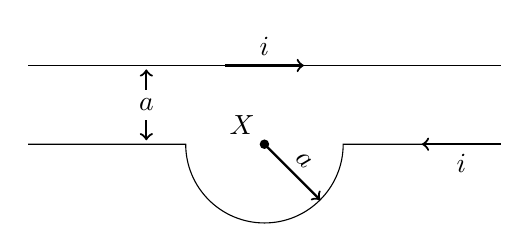
\begin{tikzpicture}
        %% top wire
        \draw (-3,1) -- (3,1);
        \draw[thick,->] (-0.5,1) -- (0.5,1) node[pos=0.5,anchor=south] {$i$};
        %% bottom wire
        \draw (-3,0) -- (-1,0) arc(180:360:1cm) -- (3,0);
        \draw[thick,->] (3,0) -- (2,0) node[pos=0.5,anchor=north] {$i$};
        %% Point X
        \draw[fill] (0,0) circle (1.5pt) node[anchor=south east] {$X$};
        \draw[thick,->] (0,0) -- (315:1cm) node[pos=0.5,anchor=south,rotate=-45] {$a$};
        %% width a
        \draw[thick,<->] (-1.5,0.05) -- (-1.5,0.95) node[pos=0.5,anchor=center,fill=white] {$a$};
    \end{tikzpicture}
    \end{center}
    What is the correct expression for the magnetic field at point $X$?
    HINT: The magnitude of the magnetic field at the center of a circular current loop of radius $R$ is $\mu_0 i/(2R)$.
    \begin{choices}
        %% NOTE: Align options with \makebox[ ]{ }
        \wrongchoice{\makebox[8em][l]{$\dfrac{\mu_0 i}{4a} + \dfrac{\mu_0 i}{2\pi a}$} out of the page}
        %% NOTE: TODO: this could  be reduced
        \wrongchoice{\makebox[8em][l]{$\dfrac{\mu_0 i}{2a} - \dfrac{\mu_0 i}{2\pi a} + \dfrac{\mu_0 i}{2\pi a}$} out of the page}
      \correctchoice{\makebox[8em][l]{$\dfrac{\mu_0 i}{4a} + \dfrac{\mu_0 i}{2\pi a}$} into the page}
        %% NOTE: TODO: this could  be reduced
        \wrongchoice{\makebox[8em][l]{$\dfrac{\mu_0 i}{4a} + \dfrac{\mu_0 i}{2\pi a} + \dfrac{\mu_0 i}{2\pi a}$} into the page}
        \wrongchoice{\makebox[8em][l]{$\dfrac{\mu_0 i}{2a} - \dfrac{\mu_0 i}{2\pi a}$} into the page}
    \end{choices}
\end{question}
}


%% PhysicsOlympiad 1994
%%----------------------------------------



\endinput


